\documentclass[thesis.tex]{subfiles}

\pagebreak
\appendix
\chapter{Example model output}
Some examples of the trained model's output are shown in Figures \ref{fig:rn-results-good} and \ref{fig:rn-results-bad}.

We can see that the model in fact performs quite well on full-sized receipts, able to capture most of their content. However, edge cases where texts are blurry, or when there's additional whitespace in the image cause a lot of struggle for the model. This suggests that more augmentation or preprocessing can improve performance.

\begin{figure}[ht!]
    \centering
    \begin{subfigure}[t]{0.45\textwidth}
        \centering
        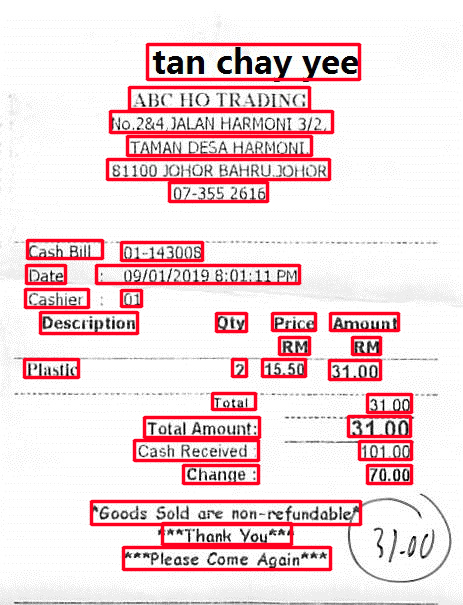
\includegraphics[width=0.45\textwidth]{rn-result-1.png}
	    \caption{Model output on a clear, full-sized receipt}  
    \end{subfigure}
    \begin{subfigure}[t]{0.45\textwidth}
        \centering
        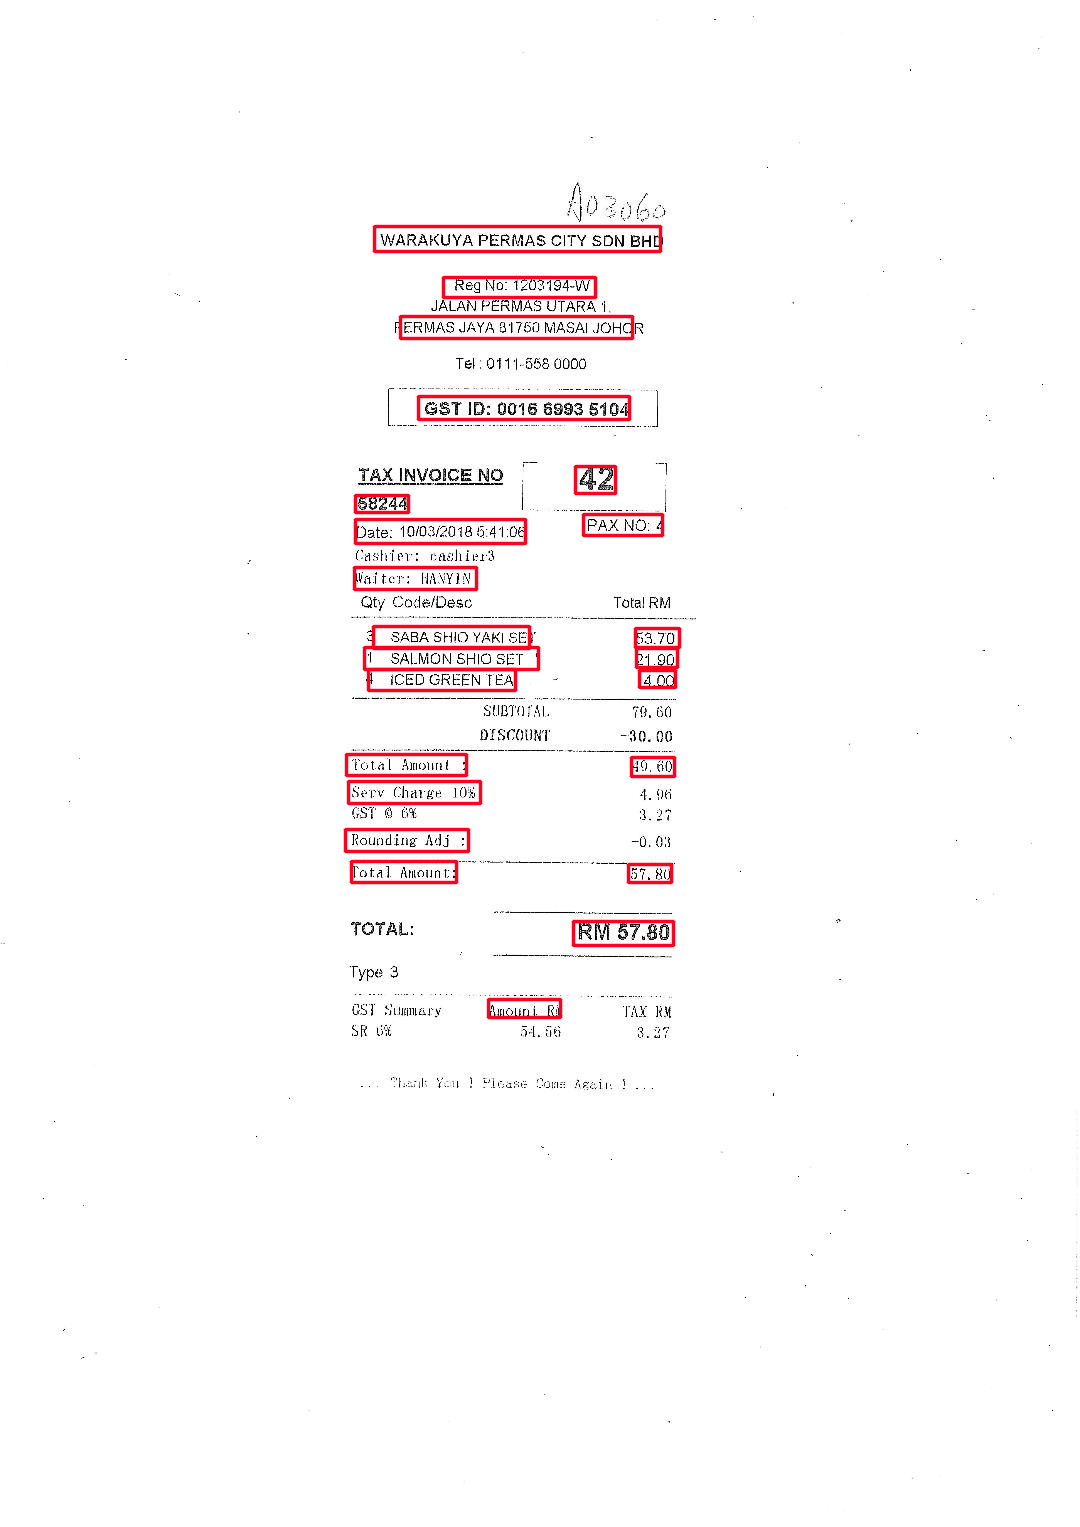
\includegraphics[width=0.45\textwidth]{rn-result-4.png}
	    \caption{Model output on a clear, full-sized receipt}  
    \end{subfigure}
    \caption{Trained model outputs with high accuracy on the validation set}
	\label{fig:rn-results-good}
\end{figure}
\FloatBarrier

\begin{figure}[ht!]
    \begin{subfigure}[t]{0.45\textwidth}
        \centering
        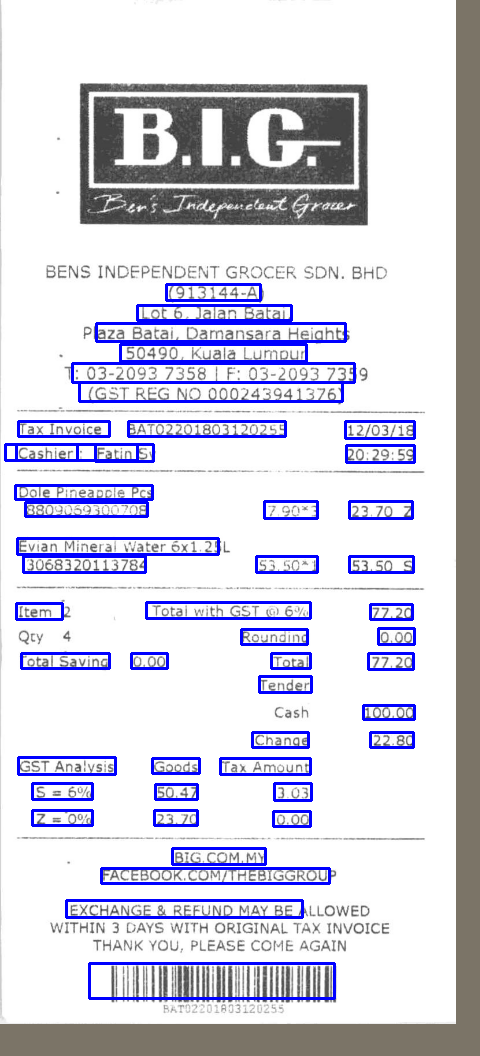
\includegraphics[width=0.45\textwidth]{rn-result-2.png}
	    \caption{Model output on a blurry receipt}
    \end{subfigure}
    \begin{subfigure}[t]{0.45\textwidth}
        \centering
        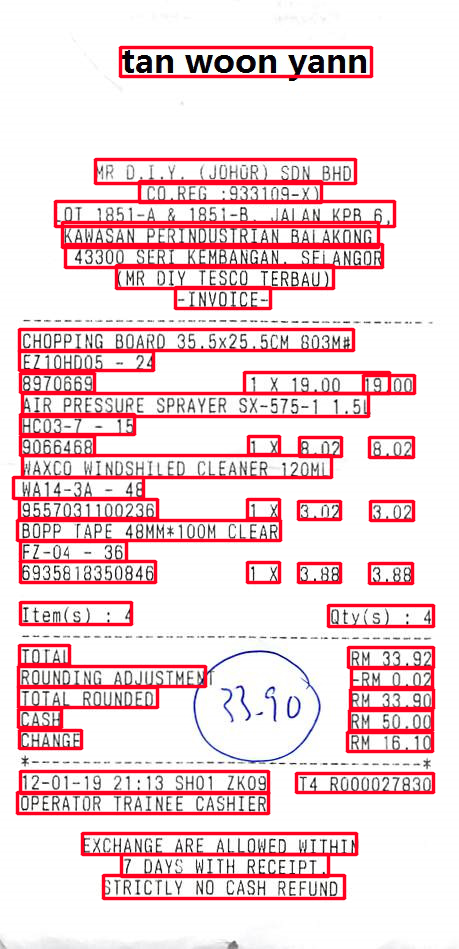
\includegraphics[width=0.45\textwidth]{rn-result-3.png}
	    \caption{Model output on a receipt with extra whitespaces}        
    \end{subfigure}
    \caption{Trained model outputs with low accuracy on the validation set}
	\label{fig:rn-results-bad}
\end{figure}
